\documentclass[8pt,aspectratio=1610]{beamer}
\usepackage[utf8]{inputenc}
\usepackage{booktabs}
\usepackage{array}
\usepackage{graphicx}
\usepackage{xcolor}
\usepackage{tikz}
\usetikzlibrary{positioning,arrows.meta,decorations.pathreplacing,calc,shadows}
\usepackage{pgfplots}
\pgfplotsset{compat=1.18}
\usepackage{amsmath}
\usepackage{amssymb}
\usepackage{amsfonts}
\usepackage{algorithm}
\usepackage{algorithmic}

\usetheme{metropolis}
\usecolortheme{wolverine}
\metroset{progressbar=frametitle,block=fill}
\setbeamertemplate{navigation symbols}{}

% Define custom colors complementing the Wolverine theme
\definecolor{maizelight}{RGB}{255, 203, 5}
\definecolor{maizedark}{RGB}{255, 167, 0}
\definecolor{bluelight}{RGB}{0, 39, 76}
\definecolor{tealaccent}{RGB}{0, 128, 128}
\definecolor{orangeaccent}{RGB}{255, 138, 51}
\definecolor{success}{RGB}{6, 167, 125}

% Customize block colors
\setbeamercolor{block title}{bg=bluelight,fg=white}
\setbeamercolor{block body}{bg=bluelight!10,fg=black}
\setbeamercolor{block title example}{bg=maizelight,fg=black}
\setbeamercolor{block body example}{bg=maizelight!15,fg=black}
\setbeamercolor{block title alerted}{bg=orangeaccent,fg=white}
\setbeamercolor{block body alerted}{bg=orangeaccent!15,fg=black}

% Custom block environments
\newenvironment<>{techblock}[1]{%
  \setbeamercolor{block title}{bg=tealaccent,fg=white}%
  \setbeamercolor{block body}{bg=tealaccent!10,fg=black}%
  \begin{block}#2{#1}}{\end{block}}

\newenvironment<>{tipblock}[1]{%
  \setbeamercolor{block title}{bg=maizedark,fg=black}%
  \setbeamercolor{block body}{bg=maizedark!15,fg=black}%
  \begin{block}#2{#1}}{\end{block}}

% Title slide information
\title{Introduction to Machine Learning}
\subtitle{CMSC 173 - Machine Learning}
\author{Noel Jeffrey Pinton}
\institute{Department of Computer Science\\University of the Philippines - Cebu}
\date{\today}

\begin{document}

\frame{\titlepage}

\begin{frame}{Course Overview}
\tableofcontents
\end{frame}

\section{What is Machine Learning?}

\begin{frame}{What is Machine Learning?}
\begin{columns}[T]
\begin{column}{0.58\textwidth}
\begin{block}{Formal Definition}
\textbf{Machine Learning (ML)} is the science of getting computers to learn and act like humans do, and improve their learning over time in autonomous fashion, by feeding them data and information.
\end{block}

\vspace{0.1cm}

\begin{block}{Key Characteristics}
\begin{itemize}
\setlength{\itemsep}{2pt}
\item \textbf{Learning from data} without explicit programming
\item \textbf{Improving performance} with experience
\item \textbf{Discovering patterns} in complex datasets
\item \textbf{Making predictions} or decisions
\end{itemize}
\end{block}
\end{column}

\begin{column}{0.40\textwidth}
\begin{exampleblock}{Traditional Programming vs ML}
\textbf{Traditional:}\\
Rules + Data $\rightarrow$ Answers

\vspace{0.2cm}

\textbf{Machine Learning:}\\
Data + Answers $\rightarrow$ Rules
\end{exampleblock}

\vspace{0.15cm}

\begin{alertblock}{Core Insight}
ML finds the rules automatically from examples!
\end{alertblock}
\end{column}
\end{columns}
\end{frame}

\begin{frame}{Historical Context}
\centering
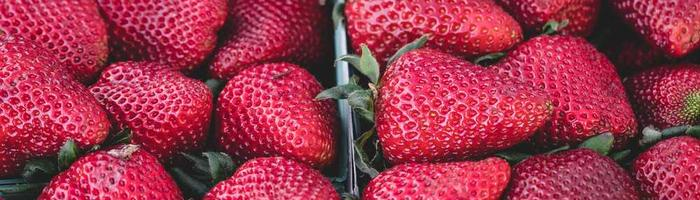
\includegraphics[width=0.75\textwidth]{../figures/aihistory.jpg}

{\small \textit{``A computer would deserve to be called intelligent if it could deceive a human into believing that it was human.''} --- Alan Turing}

\vspace{0.1cm}

\begin{columns}[T]
\begin{column}{0.48\textwidth}
\begin{block}{Major Milestones}
\begin{itemize}
\setlength{\itemsep}{2pt}
\item \textbf{1950s}: Alan Turing - "Can machines think?"
\item \textbf{1957}: Perceptron (Frank Rosenblatt)
\item \textbf{1986}: Backpropagation popularized
\item \textbf{1990s}: Support Vector Machines
\item \textbf{1997}: Deep Blue defeats Kasparov
\item \textbf{2006}: Deep Learning renaissance
\item \textbf{2012}: AlexNet wins ImageNet
\item \textbf{2016}: AlphaGo defeats Lee Sedol
\item \textbf{2020s}: Large Language Models
\end{itemize}
\end{block}
\end{column}

\begin{column}{0.48\textwidth}
\begin{exampleblock}{The Three AI Winters}
Periods of reduced funding and interest:
\begin{itemize}
\setlength{\itemsep}{2pt}
\item 1970s: Perceptron limitations
\item 1987-1993: Expert systems fail
\item Post-2000: AI hype deflation
\end{itemize}
\end{exampleblock}

\vspace{0.1cm}

\begin{alertblock}{Current Era}
We're in the \textbf{Deep Learning Revolution}:
\begin{itemize}
\setlength{\itemsep}{1pt}
\item Big data availability
\item GPU acceleration
\item Novel architectures (Transformers)
\item Widespread deployment
\end{itemize}
\end{alertblock}
\end{column}
\end{columns}
\end{frame}

\begin{frame}{Real-World Applications}
\centering
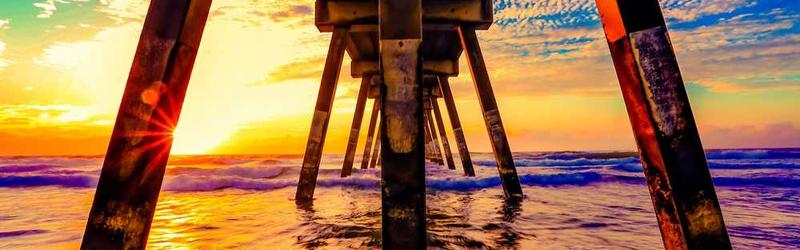
\includegraphics[width=0.85\textwidth]{../figures/mlapps.jpg}

{\small \textit{``Machine learning is the last invention that humanity will ever need to make.''} --- Nick Bostrom}

\vspace{0.1cm}

\begin{columns}[T]
\begin{column}{0.48\textwidth}
\begin{block}{Computer Vision}
\begin{itemize}
\setlength{\itemsep}{2pt}
\item Medical image diagnosis
\item Autonomous vehicles
\item Facial recognition
\item Object detection \& tracking
\item Image generation (DALL-E, Midjourney)
\end{itemize}
\end{block}

\vspace{0.08cm}

\begin{block}{Natural Language Processing}
\begin{itemize}
\setlength{\itemsep}{2pt}
\item Machine translation
\item Chatbots \& virtual assistants
\item Sentiment analysis
\item Text summarization
\item Question answering
\end{itemize}
\end{block}
\end{column}

\begin{column}{0.48\textwidth}
\begin{block}{Other Domains}
\begin{itemize}
\setlength{\itemsep}{2pt}
\item \textbf{Finance}: Fraud detection, trading
\item \textbf{Healthcare}: Drug discovery, medicine
\item \textbf{E-commerce}: Recommendations
\item \textbf{Gaming}: AI opponents
\item \textbf{Manufacturing}: Quality control
\item \textbf{Agriculture}: Crop monitoring
\end{itemize}
\end{block}

\vspace{0.08cm}

\begin{alertblock}{Impact}
ML is transforming every industry!
\end{alertblock}
\end{column}
\end{columns}
\end{frame}

\begin{frame}{Learning Objectives}
\begin{block}{By the end of this course, you will be able to:}
\begin{enumerate}
\setlength{\itemsep}{4pt}
\item \textbf{Understand} the fundamental concepts and mathematical foundations of machine learning
\item \textbf{Distinguish} between different types of learning paradigms (supervised, unsupervised, etc.)
\item \textbf{Implement} core ML algorithms from scratch using Python
\item \textbf{Apply} appropriate ML techniques to real-world problems
\item \textbf{Evaluate} model performance using rigorous metrics
\item \textbf{Analyze} the theoretical properties of learning algorithms
\item \textbf{Compare} different approaches and select optimal methods
\item \textbf{Understand} state-of-the-art techniques in deep learning
\end{enumerate}
\end{block}

\vspace{0.1cm}

\begin{alertblock}{Prerequisites}
\textbf{CMSC 170}: Linear algebra, probability theory, calculus, Python programming
\end{alertblock}
\end{frame}

\section{Types of Machine Learning}

\begin{frame}{Machine Learning Taxonomy}
\centering
\begin{tikzpicture}[
    level 1/.style={sibling distance=4.5cm, level distance=1.8cm},
    level 2/.style={sibling distance=2.8cm, level distance=1.8cm},
    every node/.style={rectangle, draw, rounded corners, text width=3.2cm, align=center, fill=bluelight!20, font=\small},
    edge from parent/.style={draw, -latex, thick, color=bluelight}
  ]

\node[fill=orangeaccent!40, text width=4cm, font=\bfseries] {Machine Learning}
  child {node {Supervised Learning}
    child {node[fill=tealaccent!20, text width=2.5cm] {Regression}}
    child {node[fill=tealaccent!20, text width=2.5cm] {Classification}}
  }
  child {node {Unsupervised Learning}
    child {node[fill=maizelight!30, text width=2.5cm] {Clustering}}
    child {node[fill=maizelight!30, text width=2.5cm] {Dimensionality Reduction}}
  }
  child {node {Others}
    child {node[fill=gray!20, text width=2.5cm] {Semi-supervised}}
    child {node[fill=gray!20, text width=2.5cm] {Reinforcement}}
  };

\end{tikzpicture}
\end{frame}

\section{Supervised Learning}

\begin{frame}{Supervised Learning}
\centering
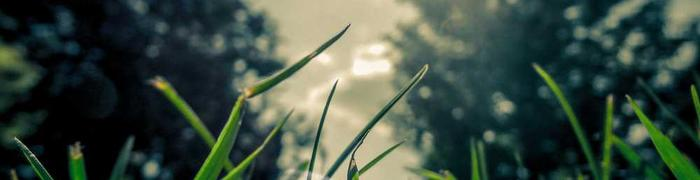
\includegraphics[width=0.75\textwidth]{../figures/supervised.jpg}

{\small \textit{``Learning is finding out what you already know. Doing is demonstrating that you know it.''} --- Richard Bach}

\vspace{0.08cm}

\begin{columns}[T]
\begin{column}{0.55\textwidth}
\begin{block}{Definition}
Learning from \textbf{labeled data} where each training example consists of:
\begin{itemize}
\setlength{\itemsep}{2pt}
\item \textbf{Input}: Feature vector $\mathbf{x} \in \mathbb{R}^d$
\item \textbf{Output}: Label/target $y$
\end{itemize}

\vspace{0.1cm}

\textbf{Goal}: Learn a function $f: \mathcal{X} \rightarrow \mathcal{Y}$ such that $f(\mathbf{x}) \approx y$
\end{block}

\vspace{0.1cm}

\begin{block}{Training Process}
Given dataset $\mathcal{D} = \{(\mathbf{x}_1, y_1), \ldots, (\mathbf{x}_n, y_n)\}$:

\begin{enumerate}
\setlength{\itemsep}{1pt}
\item Choose a hypothesis class $\mathcal{H}$
\item Define a loss function $\mathcal{L}(y, \hat{y})$
\item Minimize empirical risk:
$$\hat{f} = \arg\min_{f \in \mathcal{H}} \frac{1}{n}\sum_{i=1}^n \mathcal{L}(y_i, f(\mathbf{x}_i))$$
\item Evaluate on unseen test data
\end{enumerate}
\end{block}
\end{column}

\begin{column}{0.43\textwidth}
\begin{exampleblock}{Key Properties}
\begin{itemize}
\setlength{\itemsep}{3pt}
\item \textbf{Labeled data required}
\item \textbf{Teacher signal} guides learning
\item \textbf{Generalization} to new examples
\item \textbf{Performance measurable}
\end{itemize}
\end{exampleblock}

\vspace{0.1cm}

\begin{exampleblock}{Two Main Tasks}
\textbf{1. Regression} ($y \in \mathbb{R}$)\\
Predict continuous values

\vspace{0.15cm}

\textbf{2. Classification} ($y \in \{1,\ldots,K\}$)\\
Predict discrete categories
\end{exampleblock}

\vspace{0.1cm}

\begin{alertblock}{Challenge}
Avoid overfitting to training data!
\end{alertblock}
\end{column}
\end{columns}
\end{frame}

\begin{frame}{Regression: Predicting Continuous Values}
\centering
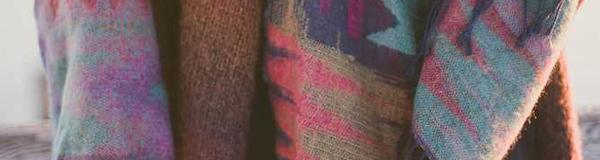
\includegraphics[width=0.65\textwidth]{../figures/regression.jpg}

{\small \textit{``All models are wrong, but some are useful.''} --- George Box}

\vspace{0.08cm}

\begin{columns}[T]
\begin{column}{0.48\textwidth}
\begin{block}{Problem Formulation}
\textbf{Input}: $\mathbf{x} \in \mathbb{R}^d$ (features)\\
\textbf{Output}: $y \in \mathbb{R}$ (continuous target)\\
\textbf{Model}: $\hat{y} = f(\mathbf{x}; \theta)$
\end{block}

\vspace{0.1cm}

\begin{block}{Common Loss Functions}
\textbf{Mean Squared Error (MSE):}
$$\mathcal{L}(\theta) = \frac{1}{n}\sum_{i=1}^n (y_i - \hat{y}_i)^2$$

\textbf{Mean Absolute Error (MAE):}
$$\mathcal{L}(\theta) = \frac{1}{n}\sum_{i=1}^n |y_i - \hat{y}_i|$$

\textbf{Huber Loss} (robust to outliers):
$$\mathcal{L}_\delta(r) = \begin{cases}
\frac{1}{2}r^2 & |r| \leq \delta \\
\delta(|r| - \frac{\delta}{2}) & |r| > \delta
\end{cases}$$
\end{block}
\end{column}

\begin{column}{0.48\textwidth}
\begin{exampleblock}{Regression Algorithms}
\begin{itemize}
\setlength{\itemsep}{3pt}
\item \textbf{Linear Regression}
\item Ridge Regression (L2 regularization)
\item Lasso Regression (L1 regularization)
\item \textbf{Polynomial Regression}
\item \textbf{Cubic Splines}
\item Support Vector Regression (SVR)
\item Decision Tree Regression
\item Neural Networks
\end{itemize}
\end{exampleblock}

\vspace{0.1cm}

\begin{exampleblock}{Real-World Examples}
\begin{itemize}
\setlength{\itemsep}{2pt}
\item House price prediction
\item Stock market forecasting
\item Temperature prediction
\item Energy consumption forecasting
\item Sales prediction
\end{itemize}
\end{exampleblock}
\end{column}
\end{columns}
\end{frame}

\begin{frame}{Classification: Predicting Categories}
\centering
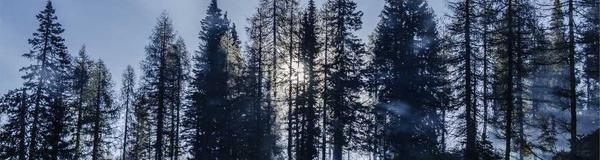
\includegraphics[width=0.65\textwidth]{../figures/classification.jpg}

{\small \textit{``The goal is to turn data into information, and information into insight.''} --- Carly Fiorina}

\vspace{0.08cm}

\begin{columns}[T]
\begin{column}{0.48\textwidth}
\begin{block}{Problem Formulation}
\textbf{Input}: $\mathbf{x} \in \mathbb{R}^d$ (features)\\
\textbf{Output}: $y \in \{1, 2, \ldots, K\}$ (class label)\\
\textbf{Model}: $\hat{y} = \arg\max_k P(y=k|\mathbf{x})$
\end{block}

\vspace{0.1cm}

\begin{block}{Types of Classification}
\textbf{Binary Classification}: $K=2$
\begin{itemize}
\setlength{\itemsep}{1pt}
\item Spam vs. not spam
\item Disease vs. healthy
\end{itemize}

\vspace{0.1cm}

\textbf{Multi-class}: $K > 2$
\begin{itemize}
\setlength{\itemsep}{1pt}
\item Digit recognition (0-9)
\item Animal species classification
\end{itemize}

\vspace{0.1cm}

\textbf{Multi-label}: Multiple categories per example
\begin{itemize}
\setlength{\itemsep}{1pt}
\item Image tagging (cat, outdoor, sunny)
\end{itemize}
\end{block}
\end{column}

\begin{column}{0.48\textwidth}
\begin{exampleblock}{Classification Algorithms}
\begin{itemize}
\setlength{\itemsep}{3pt}
\item \textbf{Logistic Regression}
\item \textbf{Naïve Bayes}
\item \textbf{K-Nearest Neighbors (KNN)}
\item \textbf{Decision Trees}
\item Support Vector Machines (SVM)
\item Random Forests
\item Gradient Boosting
\item Neural Networks
\end{itemize}
\end{exampleblock}

\vspace{0.1cm}

\begin{exampleblock}{Common Loss Functions}
\textbf{Cross-Entropy} (log loss):
$$\mathcal{L} = -\frac{1}{n}\sum_{i=1}^n \sum_{k=1}^K y_{ik} \log \hat{y}_{ik}$$

\textbf{Hinge Loss} (SVM):
$$\mathcal{L} = \max(0, 1 - y_i \hat{y}_i)$$
\end{exampleblock}
\end{column}
\end{columns}
\end{frame}

\section{Unsupervised Learning}

\begin{frame}{Unsupervised Learning}
\begin{columns}[T]
\begin{column}{0.55\textwidth}
\begin{block}{Definition}
Learning from \textbf{unlabeled data} without explicit target outputs:
\begin{itemize}
\setlength{\itemsep}{2pt}
\item \textbf{Input}: Feature vectors $\{\mathbf{x}_1, \ldots, \mathbf{x}_n\}$
\item \textbf{Output}: None (discover structure)
\end{itemize}

\vspace{0.1cm}

\textbf{Goal}: Discover hidden patterns, structures, or relationships in data
\end{block}

\vspace{0.1cm}

\begin{block}{Main Tasks}
\textbf{1. Clustering}
\begin{itemize}
\setlength{\itemsep}{1pt}
\item Group similar data points
\item Algorithms: K-Means, DBSCAN, Hierarchical
\end{itemize}

\vspace{0.1cm}

\textbf{2. Dimensionality Reduction}
\begin{itemize}
\setlength{\itemsep}{1pt}
\item Compress high-dimensional data
\item Algorithms: PCA, t-SNE, UMAP
\end{itemize}

\vspace{0.1cm}

\textbf{3. Density Estimation}
\begin{itemize}
\setlength{\itemsep}{1pt}
\item Model the data distribution
\item Algorithms: Gaussian Mixture Models
\end{itemize}
\end{block}
\end{column}

\begin{column}{0.43\textwidth}
\begin{exampleblock}{Key Characteristics}
\begin{itemize}
\setlength{\itemsep}{3pt}
\item \textbf{No labels} required
\item \textbf{Exploratory} in nature
\item \textbf{Structure discovery}
\item Performance harder to measure
\end{itemize}
\end{exampleblock}

\vspace{0.1cm}

\begin{exampleblock}{Applications}
\begin{itemize}
\setlength{\itemsep}{2pt}
\item Customer segmentation
\item Anomaly detection
\item Data visualization
\item Feature extraction
\item Compression
\item Recommender systems
\end{itemize}
\end{exampleblock}

\vspace{0.1cm}

\begin{alertblock}{Challenge}
How do we evaluate without labels?
\end{alertblock}
\end{column}
\end{columns}
\end{frame}

\begin{frame}{Clustering: Grouping Similar Data}
\centering
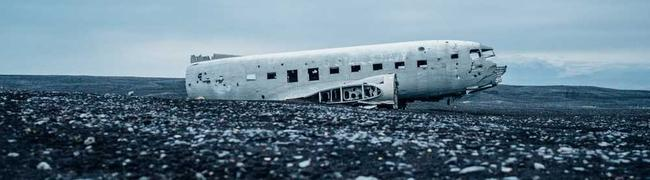
\includegraphics[width=0.70\textwidth]{../figures/clustering.jpg}

{\small \textit{``Without data, you're just another person with an opinion.''} --- W. Edwards Deming}

\vspace{0.1cm}

\begin{columns}[T]
\begin{column}{0.48\textwidth}
\begin{block}{Problem Formulation}
\textbf{Input}: Dataset $\{\mathbf{x}_1, \ldots, \mathbf{x}_n\}$\\
\textbf{Output}: Cluster assignments $\{c_1, \ldots, c_n\}$\\
\textbf{Goal}: Maximize intra-cluster similarity, minimize inter-cluster similarity
\end{block}

\vspace{0.1cm}

\begin{block}{K-Means Algorithm}
\textbf{Objective}: Minimize within-cluster variance
$$\min_{\{\mu_k\}, \{c_i\}} \sum_{i=1}^n \|\mathbf{x}_i - \mu_{c_i}\|^2$$

\textbf{Algorithm}:
\begin{algorithmic}[1]
\STATE Initialize $K$ centroids randomly
\REPEAT
\STATE Assign each point to nearest centroid
\STATE Update centroids as cluster means
\UNTIL{Convergence}
\end{algorithmic}

\textbf{Complexity}: $O(nKd)$ per iteration
\end{block}
\end{column}

\begin{column}{0.48\textwidth}
\begin{exampleblock}{Other Clustering Methods}
\textbf{Hierarchical Clustering}:
\begin{itemize}
\setlength{\itemsep}{1pt}
\item Agglomerative (bottom-up)
\item Divisive (top-down)
\item Creates dendrogram
\end{itemize}

\vspace{0.1cm}

\textbf{DBSCAN}:
\begin{itemize}
\setlength{\itemsep}{1pt}
\item Density-based
\item Finds arbitrary shapes
\item Handles noise/outliers
\end{itemize}

\vspace{0.1cm}

\textbf{Gaussian Mixture Models}:
\begin{itemize}
\setlength{\itemsep}{1pt}
\item Probabilistic clustering
\item Soft assignments
\item EM algorithm
\end{itemize}
\end{exampleblock}

\vspace{0.1cm}

\begin{exampleblock}{Evaluation Metrics}
\begin{itemize}
\setlength{\itemsep}{2pt}
\item Silhouette coefficient
\item Davies-Bouldin index
\item Calinski-Harabasz index
\end{itemize}
\end{exampleblock}
\end{column}
\end{columns}
\end{frame}

\begin{frame}{Dimensionality Reduction: Compression \& Visualization}
\centering
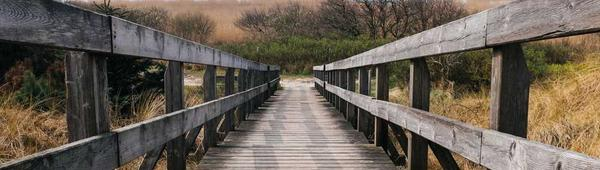
\includegraphics[width=0.65\textwidth]{../figures/dimension.jpg}

{\small \textit{``In God we trust, all others must bring data.''} --- W. Edwards Deming}

\vspace{0.08cm}

\begin{columns}[T]
\begin{column}{0.48\textwidth}
\begin{block}{Motivation}
\textbf{High-dimensional data} ($d \gg 1$) causes:
\begin{itemize}
\setlength{\itemsep}{2pt}
\item \textbf{Curse of dimensionality}
\item Computational complexity
\item Overfitting
\item Difficulty in visualization
\end{itemize}

\vspace{0.1cm}

\textbf{Solution}: Project to lower dimensions while preserving structure
\end{block}

\vspace{0.1cm}

\begin{block}{Principal Component Analysis (PCA)}
\textbf{Goal}: Find directions of maximum variance

\textbf{Method}:
\begin{enumerate}
\setlength{\itemsep}{1pt}
\item Center the data: $\tilde{\mathbf{x}}_i = \mathbf{x}_i - \bar{\mathbf{x}}$
\item Compute covariance: $\mathbf{C} = \frac{1}{n}\mathbf{X}^T\mathbf{X}$
\item Find eigenvectors of $\mathbf{C}$
\item Project onto top $k$ eigenvectors
\end{enumerate}

\textbf{Result}: $\mathbf{z}_i = \mathbf{W}^T\mathbf{x}_i$ where $\mathbf{z}_i \in \mathbb{R}^k$
\end{block}
\end{column}

\begin{column}{0.48\textwidth}
\begin{exampleblock}{Other Techniques}
\textbf{Linear Methods}:
\begin{itemize}
\setlength{\itemsep}{2pt}
\item PCA (maximum variance)
\item LDA (maximum discrimination)
\item ICA (independent components)
\end{itemize}

\vspace{0.1cm}

\textbf{Non-linear Methods}:
\begin{itemize}
\setlength{\itemsep}{2pt}
\item Kernel PCA
\item t-SNE (visualization)
\item UMAP (topology preservation)
\item Autoencoders (neural networks)
\end{itemize}
\end{exampleblock}

\vspace{0.1cm}

\begin{exampleblock}{Applications}
\begin{itemize}
\setlength{\itemsep}{2pt}
\item Data visualization (2D/3D)
\item Noise reduction
\item Feature extraction
\item Image compression
\item Preprocessing for ML
\end{itemize}
\end{exampleblock}
\end{column}
\end{columns}
\end{frame}

\section{Semi-Supervised Learning}

\begin{frame}{Semi-Supervised Learning}
\begin{columns}[T]
\begin{column}{0.55\textwidth}
\begin{block}{Definition}
Learning from \textbf{both labeled and unlabeled data}:
\begin{itemize}
\setlength{\itemsep}{2pt}
\item \textbf{Labeled}: $\mathcal{D}_L = \{(\mathbf{x}_1, y_1), \ldots, (\mathbf{x}_l, y_l)\}$
\item \textbf{Unlabeled}: $\mathcal{D}_U = \{\mathbf{x}_{l+1}, \ldots, \mathbf{x}_{l+u}\}$
\item Typically $l \ll u$ (few labels, many unlabeled)
\end{itemize}

\vspace{0.1cm}

\textbf{Goal}: Leverage unlabeled data to improve performance
\end{block}

\vspace{0.1cm}

\begin{block}{Fundamental Assumptions}
\textbf{1. Smoothness Assumption}
\begin{itemize}
\setlength{\itemsep}{1pt}
\item Nearby points share same label
\end{itemize}

\textbf{2. Cluster Assumption}
\begin{itemize}
\setlength{\itemsep}{1pt}
\item Data forms discrete clusters
\item Points in same cluster have same label
\end{itemize}

\textbf{3. Manifold Assumption}
\begin{itemize}
\setlength{\itemsep}{1pt}
\item High-dim data lies on low-dim manifold
\end{itemize}
\end{block}
\end{column}

\begin{column}{0.43\textwidth}
\begin{exampleblock}{Common Approaches}
\textbf{Self-Training}:
\begin{itemize}
\setlength{\itemsep}{1pt}
\item Train on labeled data
\item Predict unlabeled data
\item Add confident predictions to training set
\item Iterate
\end{itemize}

\vspace{0.1cm}

\textbf{Co-Training}:
\begin{itemize}
\setlength{\itemsep}{1pt}
\item Multiple views of data
\item Train separate classifiers
\item Exchange confident predictions
\end{itemize}

\vspace{0.1cm}

\textbf{Graph-Based Methods}:
\begin{itemize}
\setlength{\itemsep}{1pt}
\item Construct similarity graph
\item Propagate labels
\end{itemize}
\end{exampleblock}

\vspace{0.1cm}

\begin{alertblock}{Why Semi-Supervised?}
Labels are expensive! (Human annotation, expert knowledge, time)
\end{alertblock}
\end{column}
\end{columns}
\end{frame}

\section{Reinforcement Learning}

\begin{frame}{Reinforcement Learning}
\centering
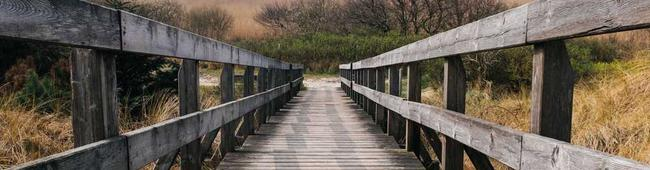
\includegraphics[width=0.70\textwidth]{../figures/robot.jpg}

{\small \textit{``You can use a spoon to eat soup, but it's better to use a ladle. Learning is choosing the right tool.''} --- Yann LeCun}

\vspace{0.08cm}

\begin{columns}[T]
\begin{column}{0.55\textwidth}
\begin{block}{Definition}
Learning through \textbf{interaction with an environment}:
\begin{itemize}
\setlength{\itemsep}{2pt}
\item \textbf{Agent} takes actions
\item \textbf{Environment} provides states \& rewards
\item \textbf{Goal}: Maximize cumulative reward
\end{itemize}
\end{block}

\vspace{0.1cm}

\begin{block}{Markov Decision Process (MDP)}
Formal framework: $(\mathcal{S}, \mathcal{A}, P, R, \gamma)$

\begin{itemize}
\setlength{\itemsep}{2pt}
\item $\mathcal{S}$: State space
\item $\mathcal{A}$: Action space
\item $P(s'|s,a)$: Transition probabilities
\item $R(s,a,s')$: Reward function
\item $\gamma \in [0,1]$: Discount factor
\end{itemize}

\vspace{0.1cm}

\textbf{Policy}: $\pi: \mathcal{S} \rightarrow \mathcal{A}$

\textbf{Value Function}:
$$V^\pi(s) = \mathbb{E}\left[\sum_{t=0}^\infty \gamma^t R_t \mid s_0=s, \pi\right]$$

\textbf{Optimal Policy}: $\pi^* = \arg\max_\pi V^\pi(s) \; \forall s$
\end{block}
\end{column}

\begin{column}{0.43\textwidth}
\begin{exampleblock}{RL vs Other Paradigms}
\textbf{Key Differences}:
\begin{itemize}
\setlength{\itemsep}{2pt}
\item No direct supervision
\item Delayed rewards
\item Exploration vs exploitation
\item Sequential decision making
\item Trial and error learning
\end{itemize}
\end{exampleblock}

\vspace{0.1cm}

\begin{exampleblock}{Classic Algorithms}
\begin{itemize}
\setlength{\itemsep}{3pt}
\item \textbf{Q-Learning}
\item SARSA
\item Policy Gradient
\item Actor-Critic
\item Deep Q-Networks (DQN)
\item Proximal Policy Optimization (PPO)
\end{itemize}
\end{exampleblock}

\vspace{0.1cm}

\begin{alertblock}{Famous Applications}
AlphaGo, robotics, game playing, autonomous driving
\end{alertblock}
\end{column}
\end{columns}
\end{frame}

\begin{frame}{RL Example: Q-Learning}
\begin{columns}[T]
\begin{column}{0.48\textwidth}
\begin{block}{Q-Learning Algorithm}
\textbf{Goal}: Learn optimal action-value function
$$Q^*(s,a) = \max_\pi \mathbb{E}\left[\sum_{t=0}^\infty \gamma^t R_t \mid s_0=s, a_0=a, \pi\right]$$

\textbf{Update Rule}:
$$Q(s,a) \leftarrow Q(s,a) + \alpha [r + \gamma \max_{a'} Q(s',a') - Q(s,a)]$$

where:
\begin{itemize}
\setlength{\itemsep}{1pt}
\item $\alpha$: Learning rate
\item $r$: Immediate reward
\item $s'$: Next state
\item $\gamma$: Discount factor
\end{itemize}

\vspace{0.1cm}

\textbf{Policy}: $\pi(s) = \arg\max_a Q(s,a)$
\end{block}
\end{column}

\begin{column}{0.48\textwidth}
\begin{block}{Algorithm Pseudocode}
\begin{algorithmic}[1]
\STATE Initialize $Q(s,a)$ arbitrarily
\FOR{each episode}
\STATE Initialize state $s$
\REPEAT
\STATE Choose action $a$ using $\epsilon$-greedy policy
\STATE Take action $a$, observe $r, s'$
\STATE $Q(s,a) \leftarrow Q(s,a) + \alpha [r + \gamma \max_{a'} Q(s',a') - Q(s,a)]$
\STATE $s \leftarrow s'$
\UNTIL{$s$ is terminal}
\ENDFOR
\end{algorithmic}
\end{block}

\vspace{0.1cm}

\begin{exampleblock}{Key Concepts}
\textbf{Exploration vs Exploitation}:
\begin{itemize}
\setlength{\itemsep}{1pt}
\item $\epsilon$-greedy: explore with probability $\epsilon$
\item Balances trying new actions vs using known good ones
\end{itemize}
\end{exampleblock}
\end{column}
\end{columns}
\end{frame}

\section{The Machine Learning Pipeline}

\begin{frame}{The ML Pipeline: From Data to Deployment}
\begin{center}
\begin{tikzpicture}[
  node distance=1.5cm and 1cm,
  box/.style={rectangle, draw, rounded corners, text width=2.8cm, align=center, fill=bluelight!20, minimum height=1.2cm, font=\small},
  arrow/.style={-latex, thick}
]

% Row 1
\node[box, fill=orangeaccent!30] (data) {1. Data Collection};
\node[box, right=of data] (clean) {2. Data Cleaning};
\node[box, right=of clean] (explore) {3. EDA};
\node[box, right=of explore] (feature) {4. Feature Engineering};

% Row 2
\node[box, below=of data] (split) {5. Train/Test Split};
\node[box, right=of split] (model) {6. Model Selection};
\node[box, right=of model] (train) {7. Training};
\node[box, right=of train] (tune) {8. Hyperparameter Tuning};

% Row 3
\node[box, below=of split] (eval) {9. Evaluation};
\node[box, right=of eval] (validate) {10. Validation};
\node[box, right=of validate] (deploy) {11. Deployment};
\node[box, right=of deploy, fill=success!30] (monitor) {12. Monitoring};

% Arrows
\draw[arrow] (data) -- (clean);
\draw[arrow] (clean) -- (explore);
\draw[arrow] (explore) -- (feature);
\draw[arrow] (feature) -- (split);
\draw[arrow] (split) -- (model);
\draw[arrow] (model) -- (train);
\draw[arrow] (train) -- (tune);
\draw[arrow] (tune) -- (eval);
\draw[arrow] (eval) -- (validate);
\draw[arrow] (validate) -- (deploy);
\draw[arrow] (deploy) -- (monitor);

% Feedback loop
\draw[arrow, dashed, orangeaccent, very thick] (monitor.south) to[bend right=45] node[below, font=\tiny] {Retrain} (model.south);

\end{tikzpicture}
\end{center}

\vspace{0.15cm}

\begin{alertblock}{Key Insight}
ML is iterative! Model performance informs feature engineering, data collection, etc.
\end{alertblock}
\end{frame}

\begin{frame}{Data Preprocessing}
\centering
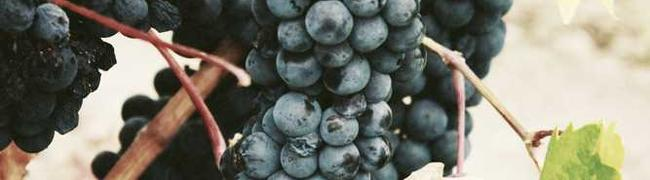
\includegraphics[width=0.70\textwidth]{../figures/dataprep.jpg}

{\small \textit{``Garbage in, garbage out.''} --- George Fuechsel}

\vspace{0.1cm}

\begin{columns}[T]
\begin{column}{0.48\textwidth}
\begin{block}{Data Cleaning}
\textbf{Common Issues}:
\begin{itemize}
\setlength{\itemsep}{2pt}
\item \textbf{Missing values}: Imputation, deletion
\item \textbf{Outliers}: Detect and handle
\item \textbf{Duplicates}: Remove
\item \textbf{Inconsistencies}: Standardize formats
\item \textbf{Noise}: Filter or smooth
\end{itemize}
\end{block}

\vspace{0.1cm}

\begin{block}{Feature Scaling}
\textbf{Why?} Many algorithms sensitive to feature scales

\textbf{Standardization} (Z-score):
$$z = \frac{x - \mu}{\sigma}$$

\textbf{Min-Max Normalization}:
$$x' = \frac{x - \min(x)}{\max(x) - \min(x)}$$

\textbf{Robust Scaling} (outlier-resistant):
$$x' = \frac{x - \text{median}(x)}{\text{IQR}(x)}$$
\end{block}
\end{column}

\begin{column}{0.48\textwidth}
\begin{block}{Feature Engineering}
\textbf{Creating new features from existing ones}:
\begin{itemize}
\setlength{\itemsep}{2pt}
\item Polynomial features: $x_1 x_2$, $x_1^2$
\item Domain-specific transformations
\item Binning continuous variables
\item One-hot encoding categorical
\item Date/time feature extraction
\item Text vectorization (TF-IDF)
\end{itemize}
\end{block}

\vspace{0.1cm}

\begin{exampleblock}{Train/Test Split}
\textbf{Why?} Evaluate generalization

\textbf{Common Splits}:
\begin{itemize}
\setlength{\itemsep}{1pt}
\item 80/20 or 70/30 train/test
\item Cross-validation (k-fold)
\item Time-series: temporal split
\end{itemize}

\vspace{0.05cm}

\textbf{Rule}: Never train on test data!
\end{exampleblock}
\end{column}
\end{columns}
\end{frame}

\begin{frame}{Model Selection \& Training}
\begin{columns}[T]
\begin{column}{0.48\textwidth}
\begin{block}{Choosing a Model}
\textbf{Consider}:
\begin{itemize}
\setlength{\itemsep}{3pt}
\item \textbf{Problem type}: Regression, classification, etc.
\item \textbf{Data size}: Deep learning needs more data
\item \textbf{Interpretability}: Linear models vs black boxes
\item \textbf{Training time}: Real-time vs offline
\item \textbf{Prediction speed}: Production requirements
\end{itemize}
\end{block}

\vspace{0.1cm}

\begin{block}{No Free Lunch Theorem}
\textbf{Theorem}: No single algorithm works best for all problems

\vspace{0.1cm}

\textbf{Implication}: Must try multiple approaches and validate empirically
\end{block}

\vspace{0.1cm}

\begin{exampleblock}{Start Simple!}
\begin{enumerate}
\setlength{\itemsep}{1pt}
\item Simple baseline (mean, majority class)
\item Linear model
\item More complex models
\item Ensemble methods
\end{enumerate}
\end{exampleblock}
\end{column}

\begin{column}{0.48\textwidth}
\begin{block}{Training Process}
\textbf{Optimization}: Minimize loss function
$$\theta^* = \arg\min_\theta \mathcal{L}(\theta; \mathcal{D})$$

\textbf{Common Optimizers}:
\begin{itemize}
\setlength{\itemsep}{2pt}
\item Gradient Descent
\item Stochastic Gradient Descent (SGD)
\item Adam (adaptive learning rate)
\item RMSprop
\end{itemize}
\end{block}

\vspace{0.1cm}

\begin{block}{Hyperparameter Tuning}
\textbf{Hyperparameters}: Set before training
\begin{itemize}
\setlength{\itemsep}{1pt}
\item Learning rate, regularization strength
\item Number of layers, hidden units
\item Tree depth, number of trees
\end{itemize}

\textbf{Search Methods}:
\begin{itemize}
\setlength{\itemsep}{1pt}
\item Grid search
\item Random search
\item Bayesian optimization
\end{itemize}
\end{block}
\end{column}
\end{columns}
\end{frame}

\begin{frame}{Model Evaluation Metrics}
\begin{columns}[T]
\begin{column}{0.48\textwidth}
\begin{block}{Regression Metrics}
\textbf{Mean Squared Error (MSE)}:
$$\text{MSE} = \frac{1}{n}\sum_{i=1}^n (y_i - \hat{y}_i)^2$$

\textbf{Root MSE (RMSE)}:
$$\text{RMSE} = \sqrt{\text{MSE}}$$

\textbf{Mean Absolute Error (MAE)}:
$$\text{MAE} = \frac{1}{n}\sum_{i=1}^n |y_i - \hat{y}_i|$$

\textbf{R-squared} (coefficient of determination):
$$R^2 = 1 - \frac{\sum_i (y_i - \hat{y}_i)^2}{\sum_i (y_i - \bar{y})^2}$$

Range: $(-\infty, 1]$, closer to 1 is better
\end{block}
\end{column}

\begin{column}{0.48\textwidth}
\begin{block}{Classification Metrics}
\textbf{Accuracy}:
$$\text{Acc} = \frac{\text{correct predictions}}{\text{total predictions}}$$

\textbf{Precision} (positive predictive value):
$$\text{Prec} = \frac{TP}{TP + FP}$$

\textbf{Recall} (sensitivity, true positive rate):
$$\text{Rec} = \frac{TP}{TP + FN}$$

\textbf{F1-Score} (harmonic mean):
$$F_1 = 2 \cdot \frac{\text{Prec} \cdot \text{Rec}}{\text{Prec} + \text{Rec}}$$

\textbf{ROC-AUC}: Area under ROC curve
\end{block}
\end{column}
\end{columns}

\vspace{0.1cm}

\begin{alertblock}{Important}
Choose metrics appropriate to your problem! Accuracy misleading for imbalanced data.
\end{alertblock}
\end{frame}

\section{Key Challenges in ML}

\begin{frame}{Bias-Variance Tradeoff}
\begin{columns}[T]
\begin{column}{0.55\textwidth}
\begin{block}{Decomposition of Expected Error}
For regression, expected test error:
$$\mathbb{E}[(y - \hat{f}(x))^2] = \text{Bias}^2 + \text{Variance} + \text{Noise}$$

\textbf{Bias}: Error from wrong assumptions
$$\text{Bias}[\hat{f}(x)] = \mathbb{E}[\hat{f}(x)] - f(x)$$

\textbf{Variance}: Error from sensitivity to training set
$$\text{Var}[\hat{f}(x)] = \mathbb{E}[(\hat{f}(x) - \mathbb{E}[\hat{f}(x)])^2]$$

\textbf{Noise}: Irreducible error $\sigma^2$
\end{block}

\vspace{0.1cm}

\begin{exampleblock}{The Tradeoff}
\begin{itemize}
\setlength{\itemsep}{2pt}
\item \textbf{Simple models}: High bias, low variance
\item \textbf{Complex models}: Low bias, high variance
\item \textbf{Goal}: Find sweet spot!
\end{itemize}
\end{exampleblock}
\end{column}

\begin{column}{0.43\textwidth}
\begin{block}{Underfitting}
\textbf{Symptoms}:
\begin{itemize}
\setlength{\itemsep}{2pt}
\item High training error
\item High test error
\item Model too simple
\end{itemize}

\textbf{Solutions}:
\begin{itemize}
\setlength{\itemsep}{2pt}
\item More features
\item More complex model
\item Less regularization
\end{itemize}
\end{block}

\vspace{0.1cm}

\begin{block}{Overfitting}
\textbf{Symptoms}:
\begin{itemize}
\setlength{\itemsep}{2pt}
\item Low training error
\item High test error
\item Model too complex
\end{itemize}

\textbf{Solutions}:
\begin{itemize}
\setlength{\itemsep}{2pt}
\item More training data
\item Regularization (L1/L2)
\item Simpler model
\item Early stopping
\item Dropout (neural networks)
\end{itemize}
\end{block}
\end{column}
\end{columns}
\end{frame}

\begin{frame}{Regularization Techniques}
\begin{columns}[T]
\begin{column}{0.48\textwidth}
\begin{block}{L2 Regularization (Ridge)}
\textbf{Modified objective}:
$$\min_\theta \mathcal{L}(\theta) + \lambda \|\theta\|_2^2$$

where $\lambda > 0$ is regularization strength

\textbf{Effect}:
\begin{itemize}
\setlength{\itemsep}{2pt}
\item Penalizes large weights
\item Shrinks coefficients toward zero
\item Improves generalization
\item Handles multicollinearity
\end{itemize}

\textbf{Closed-form solution} (linear regression):
$$\hat{\theta} = (\mathbf{X}^T\mathbf{X} + \lambda \mathbf{I})^{-1}\mathbf{X}^T\mathbf{y}$$
\end{block}
\end{column}

\begin{column}{0.48\textwidth}
\begin{block}{L1 Regularization (Lasso)}
\textbf{Modified objective}:
$$\min_\theta \mathcal{L}(\theta) + \lambda \|\theta\|_1$$

\textbf{Effect}:
\begin{itemize}
\setlength{\itemsep}{2pt}
\item Sparse solutions (some $\theta_i = 0$)
\item Automatic feature selection
\item More aggressive than L2
\end{itemize}

\textbf{No closed-form}: Use iterative methods
\end{block}

\vspace{0.1cm}

\begin{exampleblock}{Elastic Net}
\textbf{Combines L1 and L2}:
$$\min_\theta \mathcal{L}(\theta) + \lambda_1 \|\theta\|_1 + \lambda_2 \|\theta\|_2^2$$

\textbf{Benefits}:
\begin{itemize}
\setlength{\itemsep}{2pt}
\item Sparsity from L1
\item Stability from L2
\item Best of both worlds
\end{itemize}
\end{exampleblock}
\end{column}
\end{columns}
\end{frame}

\begin{frame}{The Curse of Dimensionality}
\begin{columns}[T]
\begin{column}{0.55\textwidth}
\begin{block}{Problem Statement}
As dimensionality $d$ increases:
\begin{itemize}
\setlength{\itemsep}{3pt}
\item \textbf{Volume grows exponentially}: $V \propto r^d$
\item \textbf{Data becomes sparse}: Points far apart
\item \textbf{Distance metrics break down}: All points equidistant
\item \textbf{Overfitting risk increases}: More parameters to fit
\end{itemize}
\end{block}

\vspace{0.1cm}

\begin{block}{Mathematical Insight}
In high dimensions, volume concentrated in corners:

$$\frac{V_{\text{corners}}}{V_{\text{total}}} = 1 - \left(1 - \frac{1}{2^d}\right)^{2^d} \approx 1 - e^{-1}$$

\vspace{0.1cm}

For unit hypercube, most volume is near edges!
\end{block}

\vspace{0.1cm}

\begin{exampleblock}{Data Requirements}
To maintain density, need $n \propto c^d$ samples where $c > 1$
\end{exampleblock}
\end{column}

\begin{column}{0.43\textwidth}
\begin{block}{Solutions}
\textbf{1. Dimensionality Reduction}
\begin{itemize}
\setlength{\itemsep}{1pt}
\item PCA, t-SNE, UMAP
\item Feature selection
\end{itemize}

\vspace{0.1cm}

\textbf{2. Feature Selection}
\begin{itemize}
\setlength{\itemsep}{1pt}
\item Filter methods (correlation)
\item Wrapper methods (RFE)
\item Embedded (Lasso, trees)
\end{itemize}

\vspace{0.1cm}

\textbf{3. Regularization}
\begin{itemize}
\setlength{\itemsep}{1pt}
\item L1/L2 penalties
\item Early stopping
\end{itemize}

\vspace{0.1cm}

\textbf{4. Collect More Data}
\begin{itemize}
\setlength{\itemsep}{1pt}
\item Exponentially more needed
\item Often impractical
\end{itemize}
\end{block}

\vspace{0.1cm}

\begin{alertblock}{Rule of Thumb}
$n \geq 10 \cdot d$ for reliable models
\end{alertblock}
\end{column}
\end{columns}
\end{frame}

\section{Course Structure}

\begin{frame}{CMSC 173 Course Topics}
\begin{columns}[T]
\begin{column}{0.48\textwidth}
\begin{block}{Core Foundations}
\textbf{I. Overview} (Today!)
\begin{itemize}
\setlength{\itemsep}{1pt}
\item Learning paradigms
\item Applications
\end{itemize}

\vspace{0.1cm}

\textbf{II. Parameter Estimation}
\begin{itemize}
\setlength{\itemsep}{1pt}
\item Method of Moments
\item Maximum Likelihood Estimation
\end{itemize}

\vspace{0.1cm}

\textbf{III. Regression}
\begin{itemize}
\setlength{\itemsep}{1pt}
\item Linear Regression
\item Lasso \& Ridge
\item Cubic Splines
\end{itemize}

\vspace{0.1cm}

\textbf{IV. Model Selection}
\begin{itemize}
\setlength{\itemsep}{1pt}
\item Bias-Variance Decomposition
\item Cross-Validation
\item Regularization
\end{itemize}
\end{block}
\end{column}

\begin{column}{0.48\textwidth}
\begin{block}{Advanced Methods}
\textbf{V. Classification}
\begin{itemize}
\setlength{\itemsep}{1pt}
\item Logistic Regression, Naïve Bayes
\item KNN, Decision Trees
\end{itemize}

\vspace{0.1cm}

\textbf{VI. Kernel Methods}
\begin{itemize}
\setlength{\itemsep}{1pt}
\item Support Vector Machines
\item Kernel trick
\end{itemize}

\vspace{0.1cm}

\textbf{VII. Dimensionality Reduction}
\begin{itemize}
\setlength{\itemsep}{1pt}
\item Principal Component Analysis
\end{itemize}

\vspace{0.1cm}

\textbf{VIII. Neural Networks}
\begin{itemize}
\setlength{\itemsep}{1pt}
\item Feedforward Networks
\item CNNs, Transformers
\item Generative Models
\end{itemize}

\vspace{0.1cm}

\textbf{IX. Clustering}
\begin{itemize}
\setlength{\itemsep}{1pt}
\item K-Means, Hierarchical
\item Gaussian Mixture Models
\end{itemize}
\end{block}
\end{column}
\end{columns}
\end{frame}

\begin{frame}{Learning Resources}
\begin{columns}[T]
\begin{column}{0.48\textwidth}
\begin{block}{Recommended Textbooks}
\textbf{Primary}:
\begin{itemize}
\setlength{\itemsep}{3pt}
\item Murphy, K. P. (2022). \textit{Probabilistic Machine Learning: An Introduction}. MIT Press.
\item Bishop, C. M. (2006). \textit{Pattern Recognition and Machine Learning}. Springer.
\end{itemize}

\vspace{0.1cm}

\textbf{Supplementary}:
\begin{itemize}
\setlength{\itemsep}{2pt}
\item Hastie et al. (2009). \textit{The Elements of Statistical Learning}. Springer.
\item Goodfellow et al. (2016). \textit{Deep Learning}. MIT Press.
\end{itemize}
\end{block}
\end{column}

\begin{column}{0.48\textwidth}
\begin{block}{Online Resources}
\begin{itemize}
\setlength{\itemsep}{3pt}
\item Scikit-learn documentation
\item PyTorch/TensorFlow tutorials
\item Coursera ML courses (Andrew Ng)
\item Stanford CS229 lecture notes
\item ArXiv.org for research papers
\end{itemize}
\end{block}

\vspace{0.1cm}

\begin{exampleblock}{Tools We'll Use}
\begin{itemize}
\setlength{\itemsep}{2pt}
\item Python 3.8+
\item NumPy, Pandas, Matplotlib
\item Scikit-learn
\item Jupyter Notebooks
\item PyTorch (for deep learning)
\end{itemize}
\end{exampleblock}
\end{column}
\end{columns}

\vspace{0.1cm}

\begin{alertblock}{Installation}
Ensure you have Python and required packages installed before next session!
\end{alertblock}
\end{frame}

\begin{frame}{Best Practices in Machine Learning}
\centering
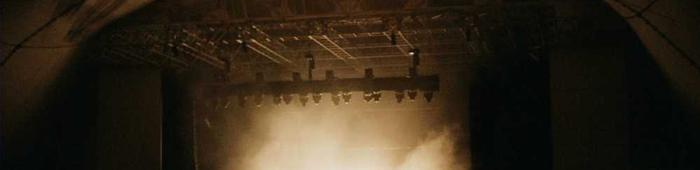
\includegraphics[width=0.75\textwidth]{../figures/workflow.jpg}

{\small \textit{``The best way to predict the future is to invent it.''} --- Alan Kay}

\vspace{0.08cm}

\begin{columns}[T]
\begin{column}{0.48\textwidth}
\begin{block}{Development Workflow}
\textbf{1. Start with baseline}
\begin{itemize}
\setlength{\itemsep}{1pt}
\item Simple model first
\item Establish minimum performance
\end{itemize}

\vspace{0.05cm}

\textbf{2. Iterate systematically}
\begin{itemize}
\setlength{\itemsep}{1pt}
\item Change one thing at a time
\item Track experiments
\item Version control (Git)
\end{itemize}

\vspace{0.05cm}

\textbf{3. Validate rigorously}
\begin{itemize}
\setlength{\itemsep}{1pt}
\item Cross-validation
\item Hold-out test set
\item Statistical significance
\end{itemize}

\vspace{0.05cm}

\textbf{4. Document everything}
\begin{itemize}
\setlength{\itemsep}{1pt}
\item Assumptions
\item Hyperparameters
\item Results
\end{itemize}
\end{block}
\end{column}

\begin{column}{0.48\textwidth}
\begin{block}{Common Pitfalls to Avoid}
\begin{itemize}
\setlength{\itemsep}{3pt}
\item \textbf{Data leakage}: Test data in training
\item \textbf{Ignoring class imbalance}
\item \textbf{Not checking for overfitting}
\item \textbf{Using wrong metrics}
\item \textbf{Not scaling features}
\item \textbf{Forgetting randomness}: Set seeds!
\item \textbf{Over-engineering}: Keep it simple
\end{itemize}
\end{block}

\vspace{0.1cm}

\begin{exampleblock}{Reproducibility}
\textbf{Essential for science}:
\begin{itemize}
\setlength{\itemsep}{2pt}
\item Set random seeds
\item Document dependencies
\item Share code \& data (when possible)
\item Report all hyperparameters
\end{itemize}
\end{exampleblock}
\end{column}
\end{columns}
\end{frame}

\begin{frame}{Ethics \& Responsible AI}
\centering
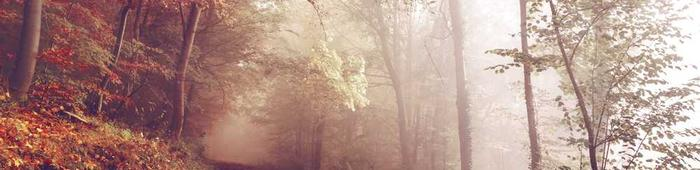
\includegraphics[width=0.75\textwidth]{../figures/ethics.jpg}

{\small \textit{``With great power comes great responsibility.''} --- Stan Lee (adapted from Voltaire)}

\vspace{0.08cm}

\begin{columns}[T]
\begin{column}{0.48\textwidth}
\begin{block}{Ethical Considerations}
\textbf{Bias \& Fairness}:
\begin{itemize}
\setlength{\itemsep}{2pt}
\item Training data may contain biases
\item Models can amplify discrimination
\item Ensure fairness across groups
\end{itemize}

\vspace{0.1cm}

\textbf{Privacy}:
\begin{itemize}
\setlength{\itemsep}{2pt}
\item Protect sensitive information
\item Anonymization techniques
\item Comply with regulations (GDPR)
\end{itemize}

\vspace{0.1cm}

\textbf{Transparency}:
\begin{itemize}
\setlength{\itemsep}{2pt}
\item Explainable AI (XAI)
\item Interpretable models
\item Document limitations
\end{itemize}

\vspace{0.1cm}

\textbf{Safety \& Security}:
\begin{itemize}
\setlength{\itemsep}{2pt}
\item Adversarial robustness
\item Prevent misuse
\item Validate thoroughly
\end{itemize}
\end{block}
\end{column}

\begin{column}{0.48\textwidth}
\begin{block}{Societal Impact}
\textbf{Positive}:
\begin{itemize}
\setlength{\itemsep}{2pt}
\item Healthcare improvements
\item Scientific discoveries
\item Accessibility tools
\item Environmental monitoring
\end{itemize}

\vspace{0.1cm}

\textbf{Concerns}:
\begin{itemize}
\setlength{\itemsep}{2pt}
\item Job displacement
\item Deepfakes \& misinformation
\item Surveillance
\item Autonomous weapons
\end{itemize}
\end{block}

\vspace{0.1cm}

\begin{alertblock}{Our Responsibility}
As ML practitioners, we must:
\begin{itemize}
\setlength{\itemsep}{1pt}
\item Consider ethical implications
\item Design inclusive systems
\item Communicate limitations
\item Prioritize societal benefit
\end{itemize}
\end{alertblock}
\end{column}
\end{columns}
\end{frame}

\section{Summary}

\begin{frame}{Key Takeaways}
\begin{block}{What We Covered Today}
\begin{enumerate}
\setlength{\itemsep}{4pt}
\item \textbf{Definition of Machine Learning}: Learning from data to improve performance
\item \textbf{Supervised Learning}: Regression \& classification with labeled data
\item \textbf{Unsupervised Learning}: Clustering \& dimensionality reduction
\item \textbf{Semi-Supervised Learning}: Leveraging both labeled \& unlabeled data
\item \textbf{Reinforcement Learning}: Learning through interaction \& rewards
\item \textbf{ML Pipeline}: From data collection to deployment
\item \textbf{Key Challenges}: Bias-variance tradeoff, overfitting, curse of dimensionality
\item \textbf{Best Practices}: Systematic development, validation, ethics
\end{enumerate}
\end{block}

\vspace{0.1cm}

\begin{alertblock}{Next Lecture}
\textbf{Parameter Estimation}: Method of Moments \& Maximum Likelihood Estimation
\end{alertblock}
\end{frame}

\begin{frame}{Prepare for Next Session}
\begin{columns}[T]
\begin{column}{0.48\textwidth}
\begin{block}{Required Reading}
\textbf{Murphy (2022)}:
\begin{itemize}
\setlength{\itemsep}{2pt}
\item Chapter 4: Statistics (4.1-4.3)
\item Chapter 5: Decision Theory (5.1-5.2)
\end{itemize}

\vspace{0.1cm}

\textbf{Bishop (2006)}:
\begin{itemize}
\setlength{\itemsep}{2pt}
\item Chapter 1: Introduction (1.1-1.5)
\item Chapter 2: Probability (2.1-2.3)
\end{itemize}
\end{block}

\vspace{0.1cm}

\begin{exampleblock}{Practice Problems}
\begin{enumerate}
\setlength{\itemsep}{2pt}
\item Review probability theory
\item Linear algebra refresher
\item Set up Python environment
\item Install required packages
\end{enumerate}
\end{exampleblock}
\end{column}

\begin{column}{0.48\textwidth}
\begin{block}{Questions to Ponder}
\begin{enumerate}
\setlength{\itemsep}{3pt}
\item When would you choose supervised vs unsupervised learning?
\item How do you decide on train/test split ratio?
\item What metrics are appropriate for imbalanced datasets?
\item How can we detect overfitting early?
\item What are ethical concerns in your domain of interest?
\end{enumerate}
\end{block}

\vspace{0.1cm}

\begin{alertblock}{Office Hours}
Available for questions and discussion after class or by appointment
\end{alertblock}
\end{column}
\end{columns}
\end{frame}

\begin{frame}[standout]
\Huge Questions?

\vspace{1cm}

\large
Thank you for your attention!

\vspace{0.5cm}

\normalsize
\textbf{Next Lecture}: Parameter Estimation\\
\textbf{See you next time!}
\end{frame}

\end{document}
